\section{Bit-flipping attack}
The subset and superset attacks described in \Cref{subsec:subset-attack} and \Cref{subsec:superset-attack} respectively, are targeting the disruption of tuples without changing the values inside the dataset. 
However, the attacker might change values by selecting some bits and flipping their values in an attempt to destroy the fingerprint.
This kind of attack is called a bit-flipping attack.
The choice of the bits is random because the attacker is modelled such that he has no knowledge about the owner's secret key that is crucial for fingerprint insertion scheme.

\subsection{AK Scheme}
Let \textit{p} be the probability that the attacker flips some $k^{\text{th}}$ least significant bit, with $p \leq 0.5$ (otherwise fingerprint detection can be applied to transformed data by flipping each fingerprintable bit back). 
The attacker chooses bits independently, therefore bit flipping is modelled as an independent Bernoulli trial with probability \text{p} of success and $1-p$ of failure. 
Assume that each fingerprint bit $f_i$ is embedded $\omega_i$ times.
The detection algorithm will fail to extract the correct fingerprint bit if the correct bit value is extracted less than the defined number of times which is controlled by parameter $\tau$.
Therefore at least $(1-\tau)\omega_i$ embedded bits must be flipped by an attacker.
Thus, the probability that the fingerprint $f$ is detected incorrectly is
\begin{equation}\label{eq:fm-bit-flipping-ak}
    fm=1-\prod_{i=0}^{L-1}(1-B(\lfloor(1-\tau)\omega_i\rfloor;\omega_i,p))
\end{equation}

Because the choice of fingerprint bits to be embedded in fingerprint embedding process is completely random, we can assume that each fingerprint bit will be embedded in the data approximately same number of times; $\omega_0=\omega_1=...=\omega_{L-1}=\omega, \forall i, j \in \{1,L-1\}, i\neq j$.
Therefore, we can write the expression for false miss rate (\Cref{eq:fm-bit-flipping-ak}) as $fm = 1 - (1-B(\lfloor(1-\tau)\omega\rfloor;\omega,p))^L$.
The results in \Cref{table:bit-flipping-ak} and \Cref{table:bit-flipping-ak-tau} are obtained using this approximation of false miss rate. 
Since $0<B(\lfloor(1-\tau)\omega\rfloor;\omega,p)\leq1$, by increasing $L$ the false miss rate also increases, meaning that longer fingerprints lead to schemes more vulnerable to bit-flipping attack.
Intuitively, longer fingerprint means fewer embeddings of each single fingerprint bit in the data and larger probability for the attacker to erase all of the embeddings of some fingerprint bit, making the detection algorithm incapable of detecting a valid fingerprint. 

The effect of parameter $\gamma$ is shown in \Cref{table:bit-flipping-ak} by calculating probabilities of success of bit-flipping attack for different values of $\gamma$ and $p$ (probability of flipping a bit, i.e. the approximate amount of tuples containing a value with a flipped bit).
We choose $\gamma=\{6, 12, 25, 50, 100, 200\}$ and $p=\{45\%, 40\%, 30\%, 20\%\}$, and set $\tau=0.5$ and $L=96$ as fixed values.
$\omega$ is calculated as $\eta/(L*\gamma)$, and $\eta=581,012$ for the convenience of comparing these results to the experimental results on Forest Covertype dataset.

\begin{table}[ht]
\centering

\caption{Probability of a successful bit-flipping attack on the AK Scheme}
\label{table:bit-flipping-ak}
\begin{tabular}{|c|c|c|c|c|} 
 \hline
   & \textbf{$p=20\%$} & \textbf{$p=30\%$} & \textbf{$p=40\%$} & \textbf{$p=45\%$} \\
 \hline
 $\gamma=6$ & 0 & 0 & $6.6530 \times 10^{-9}$ & 0.0671 \\
 \hline
 $\gamma=12$ & 0 & 0 & 0.0003 & 0.7327 \\
 \hline
 $\gamma=25$ & 0 & $5.8392\times 10^{-9}$ & 0.0941 & 0.9987 \\
 \hline
 $\gamma=50$ & 0 & 0.0002 & 0.7144 & 1 \\
 \hline
  $\gamma=100$ & $2\times 10^{-5}$ & 0.0839 & 0.9994 & 1 \\
  \hline
  $\gamma=200$ & 0.0220 & 0.8060 & 1 & 1 \\
 \hline
\end{tabular}
\end{table}

The effect of parameter $\tau$ is shown in \Cref{table:bit-flipping-ak-tau}.
The success of the bit-flipping attack is calculated for different values of $\tau$ and $p$, while $L=96$ and $\gamma=50$ are set as fixed values.

\begin{table}[ht]
\centering
\caption{Probability of a successful bit-flipping attack on the AK Scheme}
\label{table:bit-flipping-ak-tau}
\begin{tabular}{|c|c|c|c|c|} 
 \hline
 & \textbf{$p=45\%$} & \textbf{$p=40\%$} & \textbf{$p=30\%$} & \textbf{$p=20\%$} \\
 \hline
 $\tau=0.50$ & 1 & 0.7144 & 0.0002 & 0 \\
 \hline
 $\tau=0.55$ & 1 & 0.9999 & 0.0228 & 0 \\
 \hline
 $\tau=0.60$ & 1 & 1 & 0.5779 & $2\times 10^{-5}$ \\
 \hline
 $\tau=0.65$ & 1 & 1 & 1 & 0.0048 \\
 \hline
  $\tau=0.70$ & 1 & 1 & 1 & 0.3041 \\
  \hline
  $\tau=0.75$ & 1 & 1 & 1 & 0.9996 \\
 \hline
\end{tabular}
\end{table}

Both $\tau$ and $\gamma$ affect the success of the attack such that if they are increased, the probability that fingerprint will not be detected correctly is also increased, i.e. the scheme is more susceptible to bit-flipping attack.
Generally, if the attacker chooses to flip more bits, i.e. increases $p$, that also increases his chance for the successful attack, but in the same time violates credibility of the data since more original values would be changed.
Note that parameter $\xi$ does not affect the success of the attack because it is not important which LSB of a chosen value is flipped by the attacker. 

\paragraph{Misattribution false hit}
Let us now analyse the probability of detecting valid but incorrect fingerprint caused by a bit-flipping attack - misattribution false hit $fh^A$.
The detection algorithm will extract a binary bit for fingerprinting bit $f_i$ if either at most $\lfloor(1-\tau)\omega_i\rfloor-1$ or at least $\lfloor\tau\omega_i\rfloor$ of its embedded bits are flipped.
If the detection algorithm extracts a binary string, the probability that the binary string is valid but belongs to an innocent buyer is $\frac{N-1}{2^L}$.
Therefore, the probability of detecting valid but incorrect fingerprint is 
\begin{equation} \label{missattribution-false-hit-ak-bit-flipping}
    fh^A=\frac{N-1}{2^L}\prod_{i=0}^{L-1}(1-B(\lfloor(1-\tau)\omega_i\rfloor;\omega_i,p)+B(\lfloor\tau\omega_i\rfloor;\omega_i;p)).
\end{equation}

\paragraph{}
False miss rate is by definition the sum of misattribution false hit and false negative rate.
Therefore, false negative is straightforward:

\begin{equation}
\begin{aligned}
fn=& 1-\prod_{i=0}^{L-1}(1-B(\lfloor(1-\tau)\omega_i\rfloor;\omega_i,p))- \\ & \frac{N-1}{2^L}\prod_{i=0}^{L-1}(1-B(\lfloor(1-\tau)\omega_i\rfloor;\omega_i,p)+B(\lfloor\tau\omega_i\rfloor;\omega_i;p)).
\end{aligned}
\end{equation}

\paragraph{Experiments}
We have run experiments on the Forest dataset and obtained results that are shown in table \ref{table:bit-flipping-ak-emp}. 
As it is shown in the previous section, the success of bit-flipping attack is influenced by multiple parameters - length of the fingerprint \textit{L}, fingerprint detection assurance parameter $\tau$, amount of marked values $\gamma$ (or equivalently, number of embedded bits corresponding to a single bit $\omega$) and the attacker's parameter \textit{p} that defines the number of flipped bits in pirated data. 
For our experiments we fix the values of $L=96$ and $\tau=0.5$.
We run 100 experiments with different random bit-flipping pattern for each of the combinations of parameters $\gamma = {6,12,25,50,100}$ and $p={20\%,30\%,40\%,45\%}$.

\begin{table}[ht]
\centering
\caption{Experimental results of a bit-flipping attack on the AK Scheme, using the Forest Cover Type data}
\begin{tabular}{|c|c|c|c|c|} 
 \hline
 & \textbf{$p=20\%$} & \textbf{$p=30\%$} & \textbf{$p=40\%$} & \textbf{$p=45\%$} \\
 \hline
 $\gamma=6$ & 0 & 0 & 0.50 & 0.56  \\
 \hline
 $\gamma=12$ & 0  & 0 & 0.50 & 1.0 \\ 
 \hline
 $\gamma=25$ & 0  & 0 & 0.54 & 1.0  \\
 \hline
 $\gamma=50$ & 0 & 0.50 & 0.72 & 1.0   \\
 \hline
  $\gamma=100$ & 0 & 0.86 & 1.0 & 1.0  \\
 \hline
\end{tabular}
\label{table:bit-flipping-ak-emp}
\end{table}

The experimental results show that flipping 40\% of the bits available for fingerprinting most likely deletes the fingerprint. At 30\% the schemes with bigger $\gamma$ ($\gamma=50,100)$, i.e. less embedded marks, fail under the bit-flipping attack. 
Generally, the scheme is more robust against the attack for a smaller value of $\gamma$.
The empirical results differ from the analytic results in \Cref{table:bit-flipping-ak}. The two analysis agree on the cases where the attack completely succeeds and completely fails, however, in our experiments the scheme appears less robust to the bit-flipping attack than it is suggested in the analysis. 
The success rates in \Cref{table:bit-flipping-ak} are calculated using \Cref{eq:fm-bit-flipping-ak} under the assumption that all fingerprint bits are embedded the same number of times, which is approximated with $\omega$. 
This is not true due to the random nature of bit choice. In reality, every fingerprint bit has it's own $\omega_i$ value. Many fingerprint bits, thus, are embedded in data less than $\omega$ times and are easier to destroy. Since destroying all occurrences of just one fingerprint bit makes the fingerprint impossible to extract, the low occurrences of some fingerprint bits might decrease the robustness. 
This might be the reason for the difference in the attack success rates. 
Even though the probabilities for attack success are different, the boundary for robustness is confirmed. 
For $\gamma=\{6,12,25\}$ it is safe to flip up to 30\% of LSBs to not remove the fingerprint, and for larger values, $\gamma=\{50,100\}$, it is safe to flip around 20\% of the LSBs.

\subsection{Block Scheme}
Assume that the attacker examines every bit available for fingerprinting independently and selects it for flipping with probability $p$.
Let us approximate the number of times that each fingerprint bit is embedded in the data to $\omega$.
For the detection algorithm to fail to recover the correct fingerprint bit, at least $(1-\tau)\omega$ embedded bits corresponding to the single fingerprint bit $f_i$ must be changed, i.e. more than $\omega - \lceil\tau\omega\rceil+1$ bits must be changed.
Probability that one fingerprint bit is destroyed is $B(\omega-\lceil\tau\omega\rceil+1;\omega,p)$.
The probability that the entire fingerprint will be detected incorrectly is therefore 
\begin{equation}
    fm=1-(1-B(\omega-\lceil\tau\omega\rceil+1;\omega,p))^L
\end{equation}

Table \ref{table:bit-flipping-block} shows the probabilities that the bit-flipping attack will be successful on Block Scheme, depending on $p$ and $\beta$.
Parameters are set as follows: $\xi=2$, $\tau=0.5$ and $L=96$.
We choose $\eta=581012$ and $v=10$, same as Forest Covertype dataset. 

\begin{table}[ht]
    \centering
    \caption{Probability of a successful bit-flipping attack on the Block Scheme}
    \label{table:bit-flipping-block}
    \begin{tabular}{|c|c|c|c|c|}
    \hline
         & p=30\% & p=40\% & p=45\% & p=50\%\\
         \hline
        $\beta=5$ & 0 & 0 & 0 & 1.0 \\
        \hline
        $\beta=10$ & 0 & 0 & 0.02 & 1.0 \\
        \hline
        $\beta=15$ & 0 & 0.002 & 0.88 & 1.0 \\
        \hline
        $\beta=20$ & 0 & 0.017 & 0.97 & 1.0 \\
        \hline
    \end{tabular}
\end{table}


\paragraph{Experiments}
We run experiments on the Forest dataset with the previously defined parameters.
Table \ref{table:bit-flipping-block-emp} shows the obtained empirical results for the success of the bit-flipping attack on the Block Scheme.
Each experiment is run 100 times and the table shows the average success of the bit-flipping attack. 

\begin{table}[ht]
    \centering
    \caption{Experimental results of the bit-flipping attack on the Block Scheme, for the Forest Cover Type data}
    \begin{tabular}{|c|c|c|c|c|}
    \hline
         & p=30\% & p=40\% & p=45\% & p=50\%\\
         \hline
        $\beta=5$ & 0 & 0 & 0.50 & 1.0 \\
        \hline
        $\beta=10$ & 0 & 0.50 & 0.50 & 1.0 \\
        \hline
    $\beta=15$ & 0 & 0.50 & 0.92 & 1.0 \\
        \hline
        $\beta=20$ & 0.08 & 0.50 & 1.0 & 1.0 \\
        \hline
    \end{tabular}
    \label{table:bit-flipping-block-emp}
\end{table}

The experiments confirm the rule that having more marks in the data, i.e. smaller $\beta$, makes the scheme more robust against the bit-flipping attack.
Our experimental rates of the attack success, however, differ from the analytical results in \Cref{table:bit-flipping-block}. 
The change might be due to the implementation limitations introduced by the design of the Block Scheme. 
We address in \Cref{subsec:assumptions-block} the problem of "extra data" that in reality never gets fingerprinted.
This means that less data is fingerprinted, i.e. fewer marks are in the data due to this limitation than it is assumed for the calculation of the theoretical attack success rates.
This might be the reason why experimentally this scheme appears to be more vulnerable to the attack than expected by the theoretical analysis.

The scheme with all of the chosen parameters guarantees robustness for to 30\% flipped LSBs. Choosing a small value of $\beta$, e.g. 5, the tolerated amount of flipped bits rises up to 45\%.
We can argue that this is indeed a robust scheme. The assumed attacker would like to keep the data useful, and flipping more bits significantly changes the values in the data and the utility decreases.


\subsection{Two-level Fingerprinting Scheme}
In this section, we empirically analyse the robustness of the Two-level Fingerprinting Scheme against the bit-flipping attack. 
We measure the success on two levels; the ownership verification and the fingerprint extraction.
The attacker might be able to either (i) disable both ownership verification and fingerprint extraction, (ii) destroy the fingerprint but fail in disabling ownership verification, or (iii) fail in both. 
We use the Forest Covertype data for the experiments and measure success of the subset attack over 500 runs of each parameter setting. We choose: $L=96$, $\xi=2$, $\alpha_1=\alpha_2=\alpha_3=0.01$, $\gamma_1=\gamma_2=\{10,25,50,100\}$.
\Cref{fig:bit-flip-two-level-fp} shows the results of the experiments.

\begin{figure}[ht]
    \centering
    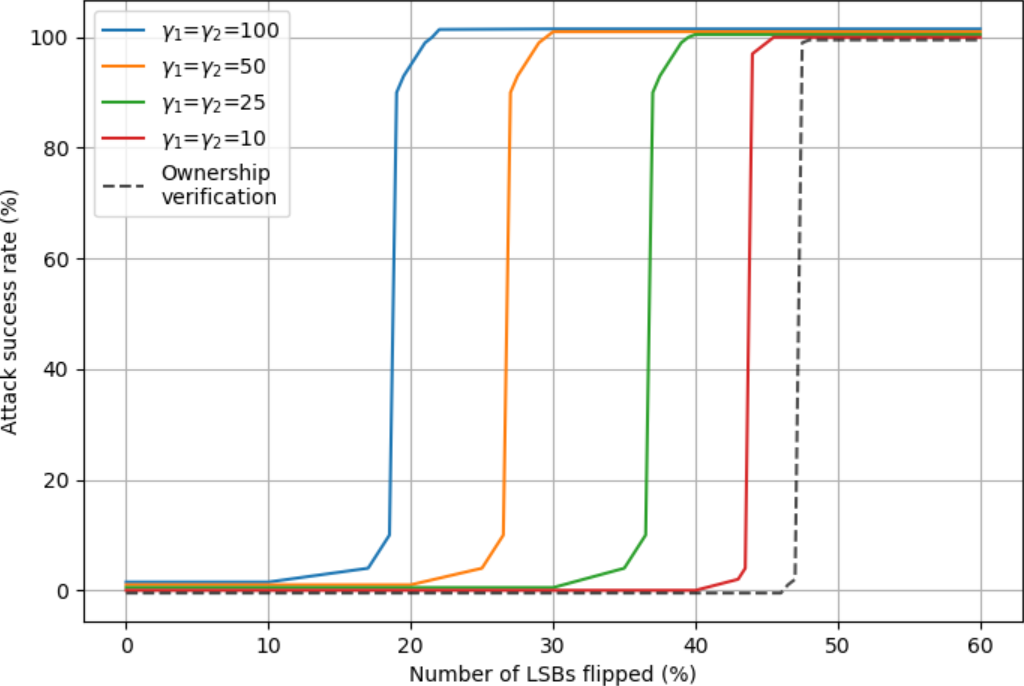
\includegraphics[width=0.9\textwidth]{Figures/bit-flip-two-level-screensh.png}
    \caption{Bit-flipping attack success in the Two-level Fingerprinting Scheme}
    \label{fig:bit-flip-two-level-fp}
\end{figure}

The coloured lines show the success rate of the attacks against the fingerprint extraction. 
The dashed line shows the success rate of the attack against the ownership verification.
The experiments show that the robustness against the bit-flipping attack, as expected, grows with more embedded marks.
The scheme with $\gamma_1=\gamma_2=100$ fails to extract the fingerprint when 19\% of the LSBs are flipped by the attacker, while the scheme with $\gamma_1=\gamma_2=10$ fails at approximately 43\% flipped LSBs.
In both cases, the ownership is verified 100\% of the times, even though the exact fingerprint cannot be extracted. 
The ownership verification fails with approximately 47\% flipped LSBs. 
The robustness of the ownership verification is very similar for each $\gamma_1$ value, therefore we represent it with only one (dashed black) line in \Cref{fig:bit-flip-two-level-fp}.

Choosing smaller $\gamma$ values makes the Two-level Fingerprinting Scheme very robust against the bit-flipping attack. The two-level fingerprint provides the additional protection measure of verifying the ownership even in cases when the exact fingerprint cannot be extracted. 
Smaller values of $\gamma$, however, introduce more error in data. How these errors affect the utility of the data, we discuss in \Cref{chapter:Utility}.